%TEX
% Sun Nov 07 12:04:37 EST 2021
% ++++++++++++++++++++++++++++++++++++++++++++++++++
% North American GeoGebra Journal LaTeX template file.  
%            :  Template Control File  
%            :  
%            :  LaTeX environment. Read the README.md file
%            :  Note configs.tex file for packages.  
%            :  MIT License.
%            :
%            : Quinlan, J. 
% ++++++++++++++++++++++++++++++++++++++++++++++++++
% FOR ASSISTANCE TRY: 
%		: http://en.wikibooks.org/wiki/LaTeX/
%		: https://www.ctan.org/
%              

\def\pagenum{1}
\def\vol{1}
\def\issue{1}

% ----------------------------- %
\documentclass[12pt]{article}


\usepackage{times}                                     
\usepackage{amsfonts,amsmath,amssymb, amsthm} 


\usepackage{latexsym}
\usepackage[a4paper]{geometry}    



\usepackage{fancyhdr}
\usepackage{placeins}                           
\usepackage{xcolor}
\usepackage[utf8]{inputenc} % Character encoding
\usepackage{graphicx}%
\usepackage{tabularx}
\usepackage{array}
\newcolumntype{x}[1]{%
>{\raggedleft\hspace{0pt}}p{#1}}%



% Book Tables
\usepackage{booktabs}



\usepackage{comment}

% USE THIS TO CHANGE THE SPACING BETWEEN TABLES AND CAPTIONS!!!
\usepackage[labelfont=bf,labelsep=period, skip=5pt]{caption}
 

% TiKz
\usepackage{pgf,tikz}
\usepackage{mathrsfs}
\usetikzlibrary{arrows}

% PDF Plots
\usepackage{pgfplots}
\pgfplotsset{width=7cm,compat=1.10}

% For side-by-side figures
\usepackage{caption}
\usepackage{subcaption}
\usepackage{float}


% Editing: highlight and strikethru
% \usepackage{soul}
% \usepackage{todonotes}  % editing (make comments \todo{X}
%\usepackage{lipsum}


% OUTLINES
\usepackage{outlines}
\usepackage{enumitem}
\setenumerate[1]{label=\arabic*.}
\setenumerate[2]{label=(\alph*).}
\setenumerate[3]{label=\roman*.}
\setenumerate[4]{label=\alph*.}

% Citations and References
% https://merkel.texture.rocks/Latex/natbib.php
\usepackage[authoryear, round]{natbib}


\makeatletter
\renewcommand\@biblabel[1]{}
\renewenvironment{thebibliography}[1]
     {\section*{\refname}%
      \@mkboth{\MakeUppercase\refname}{\MakeUppercase\refname}%
      \list{}%
           {\leftmargin0pt
            \@openbib@code
            \usecounter{enumiv}}%
      \sloppy
      \clubpenalty4000
      \@clubpenalty \clubpenalty
      \widowpenalty4000%
      \sfcode`\.\@m}
     {\def\@noitemerr
       {\@latex@warning{Empty `thebibliography' environment}}%
      \endlist}
\makeatother




\RequirePackage{color}
\definecolor{cej@color}{rgb}{0.5,0.37109375,0.59765625}
\definecolor{abs}{rgb}{0.251,0.541,0.72.9}
\definecolor{ffqqqq}{rgb}{1,0,0}
\definecolor{qqqqff}{rgb}{0,0,1}
\definecolor{cqcqcq}{rgb}{0.75,0.75,0.75}
\definecolor{ttqqqq}{rgb}{0.2,0,0}
\definecolor{ffxfqq}{rgb}{1,0.5,0}
\definecolor{uuuuuu}{rgb}{0.27,0.27,0.27}
\definecolor{ffqqff}{rgb}{1,0,1}
\definecolor{xfqqff}{rgb}{0.5,0,1}
\definecolor{xdxdff}{rgb}{0.49,0.49,1}
\definecolor{red}{rgb}{1,0,0}
\definecolor{blue}{rgb}{0,0,1}
\definecolor{ccqqqq}{rgb}{0.8,0,0}
\definecolor{fftttt}{rgb}{1,0.2,0.2}
\definecolor{qqwuqq}{rgb}{0,0.39,0}
\definecolor{qqqqff}{rgb}{0,0,1}
\definecolor{wrwrwr}{rgb}{0.3803921568627451,0.3803921568627451,0.3803921568627451}
\definecolor{sexdts}{rgb}{0.1803921568627451,0.49019607843137253,0.19607843137254902}
\definecolor{rvwvcq}{rgb}{0.08235294117647059,0.396078431372549,0.7529411764705882}
\definecolor{ccqqqq}{rgb}{0.8,0,0}
\definecolor{qqqqff}{rgb}{0,0,1}
\definecolor{wwwwww}{rgb}{0.4,0.4,0.4}
\definecolor{qqwuqq}{rgb}{0,0.39215686274509803,0}
\definecolor{uuuuuu}{rgb}{0.266,0.266,0.266}

% Allows customization of titles
\usepackage{titlesec}
\titleformat{\section}[block]{\normalsize\scshape\bfseries{\arabic{section}.}}{}{1em}{}
\titleformat{\section}[block]{\normalsize\scshape\bfseries}{\thesection}{1em}{}
\titleformat*{\subsection}{\normalsize\scshape\itshape\bfseries}
\titleformat*{\subsubsection}{\smallsize\scshape\itshape}
\usepackage{framed}
% \usepackage[hyphens]{url}
%\usepackage[hyphens,spaces,obeyspaces]{url}
% \usepackage[colorlinks,allcolors=blue]{hyperref}
\usepackage[colorlinks,allcolors=black]{hyperref}
\newtheorem{theorem}{Theorem}%[section]      
\newtheorem{acknowledgement}[theorem]{Acknowledgement}
\newtheorem{algorithm}[theorem]{Algorithm}  
\newtheorem{axiom}[theorem]{Axiom} 
\newtheorem{case}[theorem]{Case}
\newtheorem{claim}[theorem]{Claim}     %
\newtheorem{conclusion}[theorem]{Conclusion}
\newtheorem{condition}[theorem]{Condition}
\newtheorem{conjecture}[theorem]{Conjecture}
\newtheorem{corollary}[theorem]{Corollary} 
\newtheorem{criterion}[theorem]{Criterion} 
\newtheorem{definition}[theorem]{Definition}
\newtheorem{example}{Example}
\newtheorem{exercise}[theorem]{Exercise}
\newtheorem{lemma}[theorem]{Lemma}
\newtheorem{notation}[theorem]{Notation}
\newtheorem{problem}[theorem]{Problem}
\newtheorem{question}[theorem]{Question}
\newtheorem{questions}{Question}
\newtheorem{questionsa}{Question}
\newtheorem{questionsb}{Question}                   %
\newtheorem{proposition}[theorem]{Proposition}
\newtheorem{remark}[theorem]{Remark}
\newtheorem{solution}[theorem]{Solution}
\newtheorem{summary}[theorem]{Summary}



\setcounter{page}{\pagenum}
\newcounter{ggbFirstpage}
\setcounter{ggbFirstpage}{\pagenum}
\pagestyle{empty}
\setlength{\headheight}{14pt}
\geometry{left=2cm,right=2cm,top=3cm,bottom=3cm}
\pagestyle{fancyplain}                              

\fancyhf{}
\fancyhead[c]{\small \emph{Nankai University}%
\, College of Software, Machine Learning, 2013747}     %
\cfoot{%                                            
  \ifnum\value{ggbFirstpage}=\pagenum%              
    {\vtop to\hsize{\hrule\vskip .2cm {\thepage}}}%   = the starting page number         %
  \else\setcounter{ggbFirstpage}{\pagenum}\fi%      
}                                                   

\newcommand*{\TitleFont}{%
      \usefont{\encodingdefault}{\rmdefault}{}{n}%
      \fontsize{16}{18}%
      \selectfont}

\def\authorfont{\normalfont\fontsize{12}{14}\selectfont\centering}
\def\subauthorfont{\normalfont\fontsize{10}{12}\selectfont\centering}
\definecolor{wrwrwr}{rgb}{0.3803921568627451,0.3803921568627451,0.3803921568627451}
\definecolor{sexdts}{rgb}{0.1803921568627451,0.49019607843137253,0.19607843137254902}
\definecolor{rvwvcq}{rgb}{0.08235294117647059,0.396078431372549,0.7529411764705882}
\bibpunct[, ]{(}{)}{;}{a}{,}{,}


%\usepackage{mfirstuc}
% https://www.titlecase.com



 

%Display code in article
\usepackage{listings}
\usepackage{textcomp}
\usepackage{xcolor}
 \lstset{ 
  backgroundcolor=\color{white},  % background color; e.g., nearwhite you must add \usepackage{color} or \usepackage{xcolor}; should come as last argument
  basicstyle=\footnotesize\ttfamily,% the size of the fonts that are used for the code
  breakatwhitespace=false,% sets if automatic breaks should only happen at whitespace
  breaklines=true, % sets automatic line breaking
  framextopmargin=5pt,
  framexleftmargin=5pt, 
  framexbottommargin=5pt,
  framexrightmargin=0pt,
  framesep=0pt,
  captionpos=b,% sets the caption-position to bottom
  commentstyle=\color{mygreen}, % comment style
  morecomment=[s]{/*}{*/},
  deletekeywords={...}, % if want to delete keywords from the given language
  escapeinside={\%*}{*)},% if you want to add LaTeX within your code
  extendedchars=true,% lets you use non-ASCII characters; for 8-bits encodings only, does not work with UTF-8
  frame=single,	% adds a frame around the code
  keepspaces=false, % keeps spaces in text, useful for keeping indentation of code (possibly needs columns=flexible)
  keywordstyle=\color{blue},% keyword style blue
  language=java, % the language of the code
  morekeywords={},% if you want to add more keywords to the set
  numbers=none, % where line-numbers put; possible values are (none, left, right)
  numbersep=0pt,% how far the line-numbers are from the code
  numberstyle=\tiny\color{mygray}, % the style that is used for the line-numbers
  rulecolor=\color{gray},  % appleGray     % if not set, the frame-color may be changed on line-breaks within not-black text (e.g. comments (green here))
  sensitive=true,
  showspaces=false, % show spaces everywhere adding particular underscores; it overrides 'showstringspaces'
  showstringspaces=false,% underline spaces within strings only
  showtabs=false, % show tabs within strings adding particular underscores
  stepnumber=2,	% the step between two line-numbers. If it's 1, each line will be numbered
  stringstyle=\color{purple}, % string literal style
  tabsize=4,% sets default tabsize to 2 spaces
  title=\lstname, % show the filename of files included with \lstinputlisting; also try caption instead of title
  upquote=true,      % Straight quotes
  belowcaptionskip=0em,
  belowskip=0em
}

% ----------------------------- &

% 这是为了显示中文字体
\usepackage[UTF8]{ctex} % 正文中文字体
\usepackage{authblk}
\renewcommand\Authands{ and }
%\setCJKmainfont{\songti}  
%\zihao{-4}\linespread{1.5}\selectfont

% Edit 33 - 37
\def\thetitle{\uppercase{机器学习损失函数总结}} 
\def\authorOne{\authorfont{2013747张怡桢}}
\def\institutionOne{\subauthorfont{软件学院,南开大学}}

% ----------------------------- %
\begin{document}
% ----------------------------- %

\interfootnotelinepenalty=100000


% ----------------------------- %
%  Header: Title, author
% ----------------------------- %
\title{\TitleFont{\thetitle}}
\author[]{\authorOne}

\affil[]{\institutionOne}


\vspace{-1mm}
\date{}                                                 
\maketitle                                              



% ----------------------------- %
% Abstract
% ----------------------------- %
% abstract
%
\bgroup
\color{abs}
\hrule
\egroup



%
%%  DO NOT EDIT  LINES ABOVE                     %

\begin{abstract}
\noindent \textit{任务:整理典型机器学习算法的损失函数,包括线性回归、Logistic回归、带正则项的Logistic回归(岭回归)、神经网络、
线性可分SVM、带松弛变量的SVM、AdaBoost。
}\\


\noindent \textit{损失函数或者代价函数的目的是:衡量模型的预测能力的好坏。}

\noindent \textit{损失函数(Loss function):是定义在单个训练样本上的,也就是就算一个样本的误差,比如我们想要分类,就是预测的类别和实际类别的区别,是一个样本的哦,用L表示。}

\noindent \textit{代价函数(Cost function):是定义在整个训练集上面的,也就是所有样本的误差的总和的平均,也就是损失函数的总和的平均,有没有这个平均其实不会影响最后的参数的求解结果。}


%\noindent\textbf{Keywords}: Keyword1, Keyword2, Keyword3

\end{abstract}%

\bgroup
\color{abs}
\hrule
\egroup



\thispagestyle{fancy}


% ----------------------------- %
% Sections
% ----------------------------- %
% ----------------------------- %
% Author Guidelines
% ----------------------------- %


\section{损失函数(Loss function)}
\noindent 损失函数分为:经验风险损失函数;结构风险损失函数
\begin{outline}
\1经验风险损失函数:预测结果和实际结果之间的差别

\1 结构风险损失函数:经验风险损失函数 + 正则项(L0、L1(Lasso)、L2(Ridge))。

\end{outline}

\noindent 损失函数的选择依据:
\begin{outline}
	\1 采用的机器学习算法;
	\1 是否易于求导;
	\1 数据集中异常值所占的比例。
\end{outline}


\noindent 回归损失函数:MAE,MSE,RMSE,Huber Loss,Log-Cosh,Quantile Loss

\noindent 分类损失函数:log loss,CE,KL divergence,logistic loss,Focal loss,Hinge loss,Exponential loss

\subsection{回归损失函数}
\begin{outline}
	\1 平均绝对误差 MAE(Mean Absolute Error, L1 loss)
	\begin{equation}\label{loss:1}
		M A E=\frac{1}{N} \sum_{i=1}^{N}\left|y_{i}-f\left(x_{i}\right)\right|
	\end{equation}
	\2 MAE只计算误差的平均模长,而不考虑方向。

	\2 优点:所有样本对平均值的残差的权重都相同,因此对异常点更鲁棒

	\2 缺点:MAE的导数恒定,即使一个很小的误差,梯度也很大,不利于网络收敛。


	\1 平方误差(Square loss)
	\begin{equation}
		L(Y, f(x))=(Y-f(x))^{2}
	\end{equation}
	当样本个数为n时,此时的损失函数变为:
	\begin{equation}
		L(Y, f(x))=\sum_{i=1}^{n}(Y-f(x))^{2}
	\end{equation}
	Y-f(x)表示的是残差,整个式子表示的是残差的平方和,而我们的目的就是最小化这个目标函数值
	(注:该式子未加入正则项),也就是最小化残差的平方和(residual sum of squares,RSS)。
	
	而在实际应用中,通常会使用均方差(MSE)作为一项衡量指标。
	\1 均方误差 MSE(Mean Squared Error, L2 loss)
	\begin{equation}\label{loss:2}
		M S E=\frac{1}{N} \sum_{i=1}^{N}\left(y_{i}-f\left(x_{i}\right)\right)^{2}
		\end{equation}
	\2 MSE只考虑误差的平均大小,而不考虑其方向。

	\2 优点:各点都连续光滑,梯度容易计算,具有较为稳定的解

	\2 缺点:①若误差>1,在MSE中经过平方之后会进一步增大误差。如果样本中存在离群点,那么MSE的值受离群点的影响比MAE大,也就是鲁棒性不好。②当函数的输入值距离中心值较远的时候,使用梯度下降法求解的时候梯度很大,可能导致梯度爆炸。

	\1 均方根误差 RMSE(Root Mean Squared Error)
	\begin{equation}\label{loss:3}
		R M S E=\sqrt{\frac{1}{N} \sum_{i=1}^{N}\left(y_{i}-f\left(x_{i}\right)\right)^{2}}
		\end{equation}
		\2 优点:相对于MSE,RMSE的量纲和输入数据一样,比较起来更直观

		\2 缺点:受异常值影响大;梯度爆炸

	\1 Smooth L1
	\2 smooth L1说的是光滑之后的L1,前面说过了L1损失的缺点就是有折点,不光滑,导致不稳定,那如何让其变得光滑呢?smooth L1损失函数为:
	\begin{equation}\label{loss:4}
		\operatorname{smooth}_{L_{1}}(Y \mid f(x))= \begin{cases}\frac{1}{2}(Y-f(x))^{2} & |\mathrm{Y}-\mathrm{f}(\mathrm{x})|<1 \\ |Y-f(x)|-\frac{1}{2} & |\mathrm{Y}-\mathrm{f}(\mathrm{x})|>=1\end{cases}
		\end{equation}
		\2 优点:

		\3 相比于L1损失函数,函数更平滑稳定,可以收敛地更快。
		\3 相比于L2损失函数,对离群点、异常值不敏感,梯度变化相对更小,训练时不容易跑飞。
	\1 Huber Loss
	\begin{equation}\label{loss:5}
		\operatorname{Huber Loss}_{L}(Y \mid f(x))= \begin{cases}\frac{1}{2}(Y-f(x))^{2} & |\mathrm{Y}-\mathrm{f}(\mathrm{x})|<=\delta \\ \delta|Y-f(x)|-\frac{1}{2} \delta^{2} & |\mathrm{Y}-\mathrm{f}(\mathrm{x})|>\delta\end{cases}
		\end{equation}
	\2 huber损失是平方损失和绝对损失的综合,它克服了平方损失和绝对损失的缺点,不仅使损失函数具有连续的导数,而且利用MSE梯度随误差减小的特性,可取得更精确的最小值。
	\2 尽管huber损失对异常点具有更好的鲁棒性,但是,它不仅引入了额外的参数,而且选择合适的参数比较困难,这也增加了训练和调试的工作量。



		
\end{outline}

\subsection{分类损失函数}

\noindent 对于二分类问题,$y\in \{-1,+1\}$,损失函数常表示为关于 $ yf(x)$的单调递减形式。如图1:
\begin{figure}[h!] %  figure placement
    \centering
    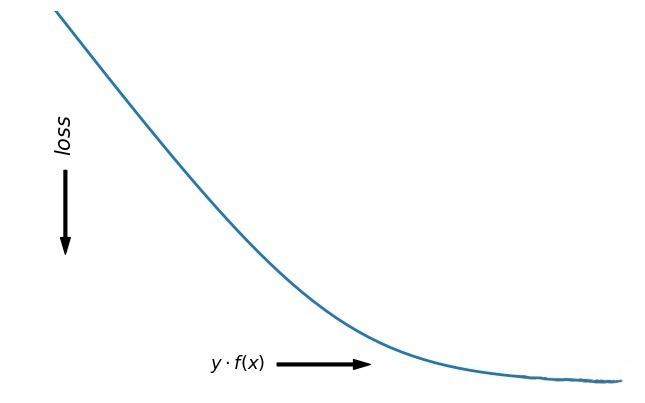
\includegraphics[scale=0.35]{figs/1.jpg} 
    \caption{二分类问题的损失函数经典表示$ yf(x)$}
    \label{fig:loss}
 \end{figure}

 \noindent $yf(x)$被称为margin,其作用类似于回归问题中的残差$y-f(x)$。

 \noindent  二分类问题中的分类规则通常为
 \begin{equation}\label{loss:6}
	\operatorname{sgn}(f(x))=\left\{\begin{array}{lll}
	+1 & \text { if } & y f(x) \geq 0 \\
	-1 & \text { if } & y f(x)<0
	\end{array}\right.
	\end{equation}
\noindent  可以看到如果$yf(x)>0$,则样本分类正确,$yf(x)<0$则分类错误,
而相应的分类决策边界即为$f(x)=0$。所以最小化损失函数也可以看作是最大化 margin 的过程,
任何合格的分类损失函数都应该对 margin<0 的样本施以较大的惩罚。



\begin{outline}
	\1 0-1损失函数
	\begin{equation}\label{loss:7}
		L(y, f(x))=\left\{\begin{array}{lll}
		0 & \text { if } \quad yf(x) \geq 0 \\
		1 & \text { if } \quad y f(x)<0
		\end{array}\right.
		\end{equation}
		\2 0-1损失对每个错分类点都施以相同的惩罚,
		这样那些“错的离谱“ (即margin→$\pm\infty $)的点并不会收到大的关注,
		这在直觉上不是很合适。感知机就是用的这种损失函数,
		但是由于相等这个条件太过严格,我们可以放宽条件,即满足 $|Y−f(x)|<T$时认为相等。
		\begin{equation}\label{loss:8}
			L(Y, f(x))=\left\{\begin{array}{lll}
			1 &\text { if } \quad |Y-f(x)| \geq T \\
			0 &\text { if } \quad |Y=f(x)|<T
			\end{array}\right.
			\end{equation}

		\2 但是0-1损失不连续、非凸,优化困难,因而常使用其他的代理损失函数进行优化。

   \1 Cross-Entropy Loss(交叉熵 Loss )
	\begin{figure}[h!]%  figure placement
    \centering
    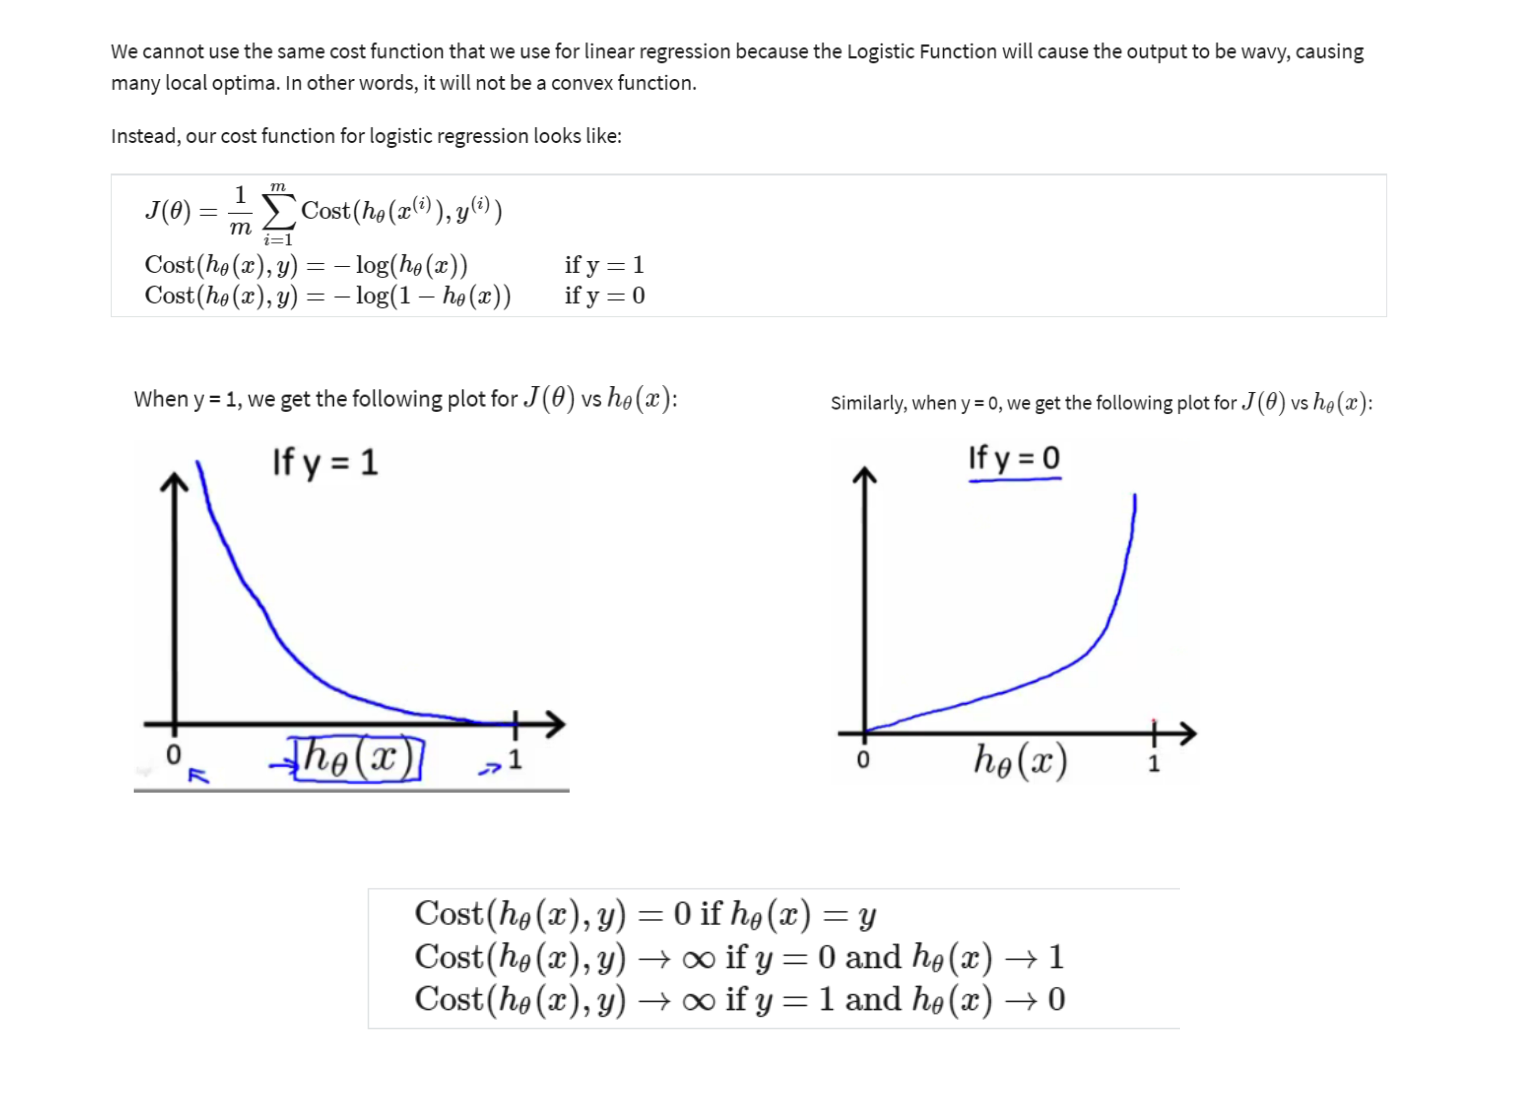
\includegraphics[scale=0.7]{figs/2.png} 
    \caption{基于吴恩达老师讲解的的交叉熵 Loss}
	\label{fig:cross}
 \end{figure}


 \noindent 二分类问题的交叉熵 Loss 主要有两种形式(标签y的定义不同):
 \2 基于输出标签 label 的表示方式为 \{0,1\},这种的就是下页图2吴恩达老师分析的形式
 \begin{equation}\label{loss:9}
	\begin{aligned}
		Loss(h_{\theta}(x_{(i)}),y_{(i)})=-y_{(i)}\log h_{\theta}(x_{(i)})-(1-y_{(i)})\log(1-h_{\theta}(x_{(i)}))
	\end{aligned}
	\end{equation}

	另有常见表达式如
	\begin{equation}\label{loss:10}
	-\sum_{i} \hat{y} \log \left(y_{i}\right)
	\end{equation}

	\begin{equation}\label{loss:11}
	L=-[y \log \hat{y}+(1-y) \log (1-\hat{y})]
	\end{equation}

	\2 基于输出标签 label 的表示方式为 \{-1,+1\} (Logistics Loss),也比较常见。它的 Loss 表达式为:
   \begin{equation}\label{loss:12}
	L(y, f(x))=\log \left(1+e^{-y f(x)}\right)
   \end{equation}
	$yf(x)$ 的符号反映了预测的准确性。


		\begin{figure}[h!]%  figure placement
    \centering
    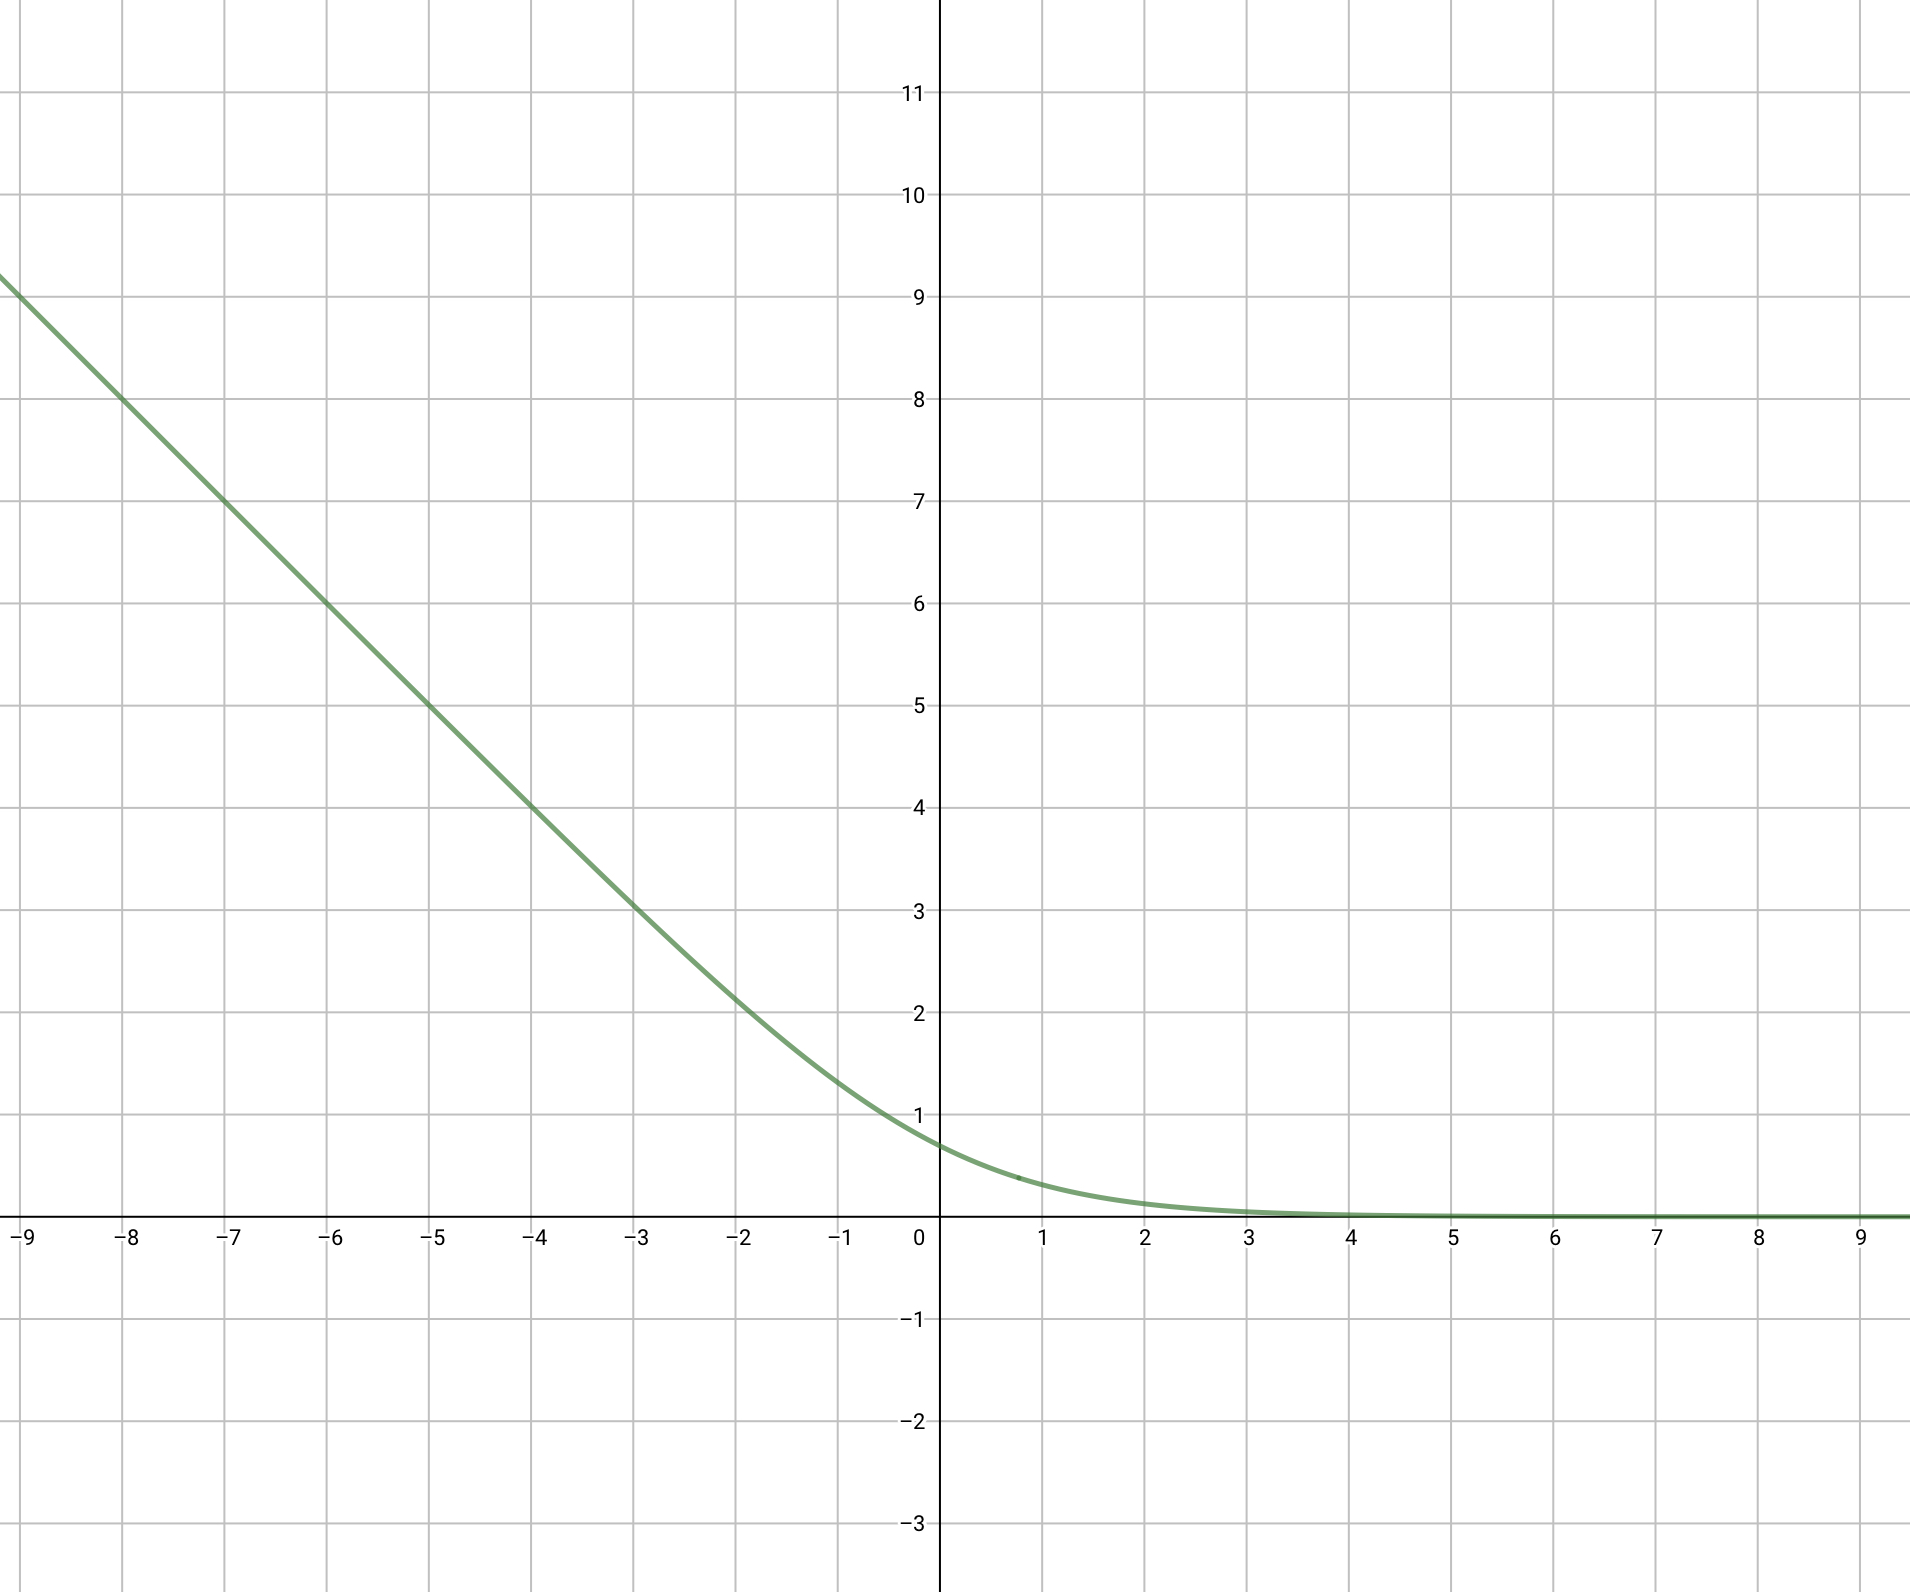
\includegraphics[scale=0.12]{figs/3.jpg} 
    \caption{绘制的$\ln \left(1+e^{-x}\right)$图}
	\label{fig:cross2}
 \end{figure}

 由下页图3可知,$yf(x)$ 同号则Loss值很小,异号则Loss很大,可以很好得表达偏差值



 \1 Log Loss(对数损失)

 \begin{equation}\label{loss:13}
	L=-\sum_{i=1}^{N} \sum_{j=1}^{C} y_{i j} \log \left(p_{i j}\right)
 \end{equation}
 其中N代表样本数量,C代表类别数, $ y_{i j}$代表第i个样本属于第j类的真实标签,$p_{i j}$表示第i个样本属于第j类的预测概率。
 
 log函数在趋近于0的时候值很大,一般要对其做clip处理。
 
 运用 log loss 的典型分类器是 Logistic 回归算法,且均可用于multi lable和multi class分类。
 
 \1 Focal loss

	$\alpha $控制类别不平衡, $\gamma $调节困难样本权重
 \begin{equation}\label{loss:14}
	\text { FocalLoss }=-\alpha\left(1-p_{t}\right)^{\gamma} \log p_{t}
 \end{equation}


\1 Hinge loss
 
 \begin{equation}\label{loss:15}
	L(y, f(x))=\max (0,1-y \times f(x))
 \end{equation}

 Hinge loss 通常被用于最大间隔算法(maximum-margin),而最大间隔算法又是SVM用到的重要算法
 
 (注意:SVM的学习算法有两种解释:1. 间隔最大化与拉格朗日对偶;2. Hinge Loss)。

	Hinge loss 专用于二分类问题,标签值y= ±1,预测值$\hat{y}\in R$。
	
	\2 当$\hat{y}\geq  +1$ 或者$\hat{y}\leq -1$时,都是分类器确定的分类结果,此时的损失函数 loss 为 0;
	
	\2 而当预测值 $\hat{y}\in$(−1,1) 时,分类器对分类结果不确定,loss 不为 0。
	显然,当$\hat{y}$= 0 时,loss 达到最大值。

\1 Exponential Loss( 指数损失 )
\begin{equation}\label{loss:16}
	L(y, f(x))=e^{-y f(x)}
 \end{equation}

 exponential loss为AdaBoost中使用的损失函数,使用exponential loss能比较方便地利用加法模型推导出AdaBoost算法。
 然而其和squared loss一样,对异常点敏感,不够robust。
\end{outline}













\section{代价函数}

\subsection{线性回归 Linearal Regression }
\begin{outline}

	\1 损失函数
		\2 利用的是平方误差的$\frac{1}{2}$倍
		\2 这里出现$\frac{1}{2}$是因为后面会有求导的步骤
	\begin{equation}\label{eq:1}
		\begin{aligned}
			Loss(h_{\theta}(x_{(i)}),y_{(i)})=\frac{1}{2}(h_{\theta }(x_{(i)})-y_{(i)})^{2}\\
		\end{aligned}
	\end{equation}

	\1 代价函数
	\2将上面式子的损失函数均方误差
	\begin{equation}\label{eq:2}
		\begin{aligned}
			\mathcal{J} (\theta )
			&=\frac{1}{m}\sum_{i=1}^{m}Loss(h_{\theta}(x_{(i)}),y_{(i)})\\
			&=\frac{1}{2m}\sum_{i = 1}^{m}(h_{\theta }(x_{(i)})-y_{(i)})^{2}\\
		\end{aligned}
	\end{equation}

	\1 带正则项的代价函数
	\begin{equation}\label{eq:3}
		\mathcal{J} (\theta )=\frac{1}{2m}[\sum_{i = 1}^{m}(h_{\theta }(x_{(i)})-y_{(i)})^{2}+\lambda \sum_{j = 1}^{n} \theta_{j}^{2} ]
\end{equation}
\end{outline}

 


% ----------------------------- %
% Logistic回归
% ----------------------------- %
\subsection{Logistic回归}
\begin{outline}
	
	\1 损失函数
	\2 这里利用的是Cross-Entropy Loss(交叉熵 Loss )的损失函数
\begin{equation}\label{eq:4}
	\begin{aligned}
		Loss(h_{\theta}(x_{(i)}),y_{(i)})=-y_{(i)}\log h_{\theta}(x_{(i)})-(1-y_{(i)})\log(1-h_{\theta}(x_{(i)}))
	\end{aligned}
\end{equation}

\1 代价函数
\2 对损失函数做均值就是Logistic回归的代价函数
\begin{equation}\label{eq:5}
	\begin{aligned}
		\mathcal{J} (\theta )
		&=\frac{1}{m}\sum_{i=1}^{m}Loss(h_{\theta}(x_{(i)}),y_{(i)})\\
		&=-\frac{1}{m}[\sum_{i = 1}^{m}y_{(i)}\log h_{\theta}(x_{(i)})+(1-y_{(i)})\log(1-h_{\theta}(x_{(i)}))]\\
	\end{aligned}
\end{equation}

\1 带正则项的代价函数
\begin{equation}\label{eq:6}
		\mathcal{J} (\theta )=[-\frac{1}{m}[\sum_{i = 1}^{m}y_{(i)}\log h_{\theta}(x_{(i)})+(1-y_{(i)})\log(1-h_{\theta}(x_{(i)}))]]+\frac{\lambda }{2m}\sum_{j = 1}^{n} \theta_{j}^{2}
\end{equation}

\end{outline}



% ----------------------------- %
% 神经网络
% ----------------------------- %
\subsection{神经网络}
\begin{outline}
	\1 基于交叉熵的代价函数
	\begin{equation}\label{eq:7}
		\begin{aligned}
		J(\Theta)=&-\frac{1}{m} \sum_{t=1}^{m} \sum_{k=1}^{K}\left[y_{k}^{(t)} \log \left(h_{\Theta}\left(x^{(t)}\right)\right)_{k}+\left(1-y_{k}^{(t)}\right) \log \left(1-h_{\Theta}\left(x^{(t)}\right)_{k}\right)\right]\\
		&+\frac{\lambda}{2 m} \sum_{l=1}^{L-1} \sum_{i=1}^{s_{l}} \sum_{j=1}^{s_{l}+1}\left(\Theta_{j, i}^{(l)}\right)^{2}
	\end{aligned}
	\end{equation}

	\1 基于平方误差的损失函数
	\begin{equation}\label{eq:8}
		E_{k}=\frac{1}{2} \sum_{k=1}^{m} \sum_{j=1}^{l}\left(\hat{y}_{j}^{k}-y_{j}^{k}\right)^{2}
	\end{equation}

\end{outline}



% ----------------------------- %
% 线性可分SVM
% ----------------------------- %
\subsection{线性可分SVM}
\begin{outline}
	\1 代价函数(拉格朗日乘子法)
\begin{equation}\label{eq:9}
	L(\mathbf{w}, b, \alpha)=\frac{1}{2}\|\mathbf{w}\|^{2}+\sum_{i=1}^{m} \alpha_{i}\left(1-y_{i}\left(\mathbf{w}^{T} \mathbf{x}_{i}+b\right)\right)
\end{equation}
\2 经验风险部分为
$\sum_{i=1}^{m} \alpha_{i}\left(1-y_{i}\left(\mathbf{w}^{T} \mathbf{x}_{i}+b\right)\right)$

而  $\mathbf{w}^{T} \mathbf{x}_{i}+b $ 应该$  \geq 1  $或 $ \leq-1 $,
最理想的是 $ y_{i}  $和 $ \mathbf{w}^{T} \mathbf{x}_{i}+b  $输出相同,损失为 0 。
\2 结构风险部分为$\frac{1}{2}\|\mathbf{w}\|^{2}$

\3 如何理解双竖线:$\frac{1}{2}\|\mathbf{w}\|^{2}=\frac{1}{2} \sum_{j=1}^{n} \mathbf{w}^{2}$

\3 结构风险公式的来源:

1. 点到直线距离 : $\frac{\left|\mathbf{w}^{T} \mathbf{x}+b\right|}{\|\mathbf{w}\|} $
所以,  $\mathbf{w}^{T} \mathbf{x}+b=1  $上的点到  $\mathbf{w}^{T} \mathbf{x}+b=0  $是$  \frac{1}{\|\mathbf{w}\|}  $。

2. 所以$\frac{2}{\|w\|} $ : 两类样本间的margin —— 我们要最大化margin才可以取得较好的分类器,这里是未使用拉格朗日乘子法的代价函数
\begin{equation}
	\begin{aligned}
		\max _{\mathbf{w}, b} &\frac{2}{\|\mathbf{w}\|}\\
s.t.   \quad  & {y_{i}\left(\mathbf{w}^{\mathrm{T}} \mathbf{x}_{i}+b\right) \geqslant 1},\\
&i=1,2,3...,m
	\end{aligned}
\end{equation}

3. 利用拉格朗日乘子法把最大化问题变成最小化的问题
\begin{equation}
	\max _{\mathbf{w}, b} \frac{2}{\|\mathbf{w}\|}\Longrightarrow \min _{\mathbf{w}, b}\frac{1}{2}\|\mathbf{w}\|^{2}
\end{equation}

结构风险与正则化形式类似,都是为了避免overfitting,因为要保证泛化能力。

知识向量机的最厉害的的地方:把结构风险与最大化间隔建立联系,也即做到最大化间隔就可以保证泛化能力。

\1 判决函数

使用训练集优化上述的代价函数,得到模型参数w,b后有如下的判决函数,判决函数的界限可以不是$\pm 1$,这取决于你对于准确的度的拿捏。
\begin{equation}
	f\left(\mathbf{x}_{i} ; \mathbf{w}\right)=\left\{\begin{array}{cc}
		1, & \mathbf{w}^{T} \mathbf{x}_{i}+b \geq 1 \\
		-1, & \mathbf{w}^{T} \mathbf{x}_{i}+b \leq-1
		\end{array}\right.
\end{equation}
对代价函数进行优化的优化模型:
\begin{equation}
	\max _{\alpha}\left\{\min _{\mathbf{w}, b} L(\mathbf{w}, b, \alpha)\right\}
\end{equation}
通过对w,b的求导以及对于$\alpha$的KKT求解之后,判决函数变成
\begin{equation}
	\begin{aligned}
		f(\mathbf{x}) &=\operatorname{sign}\left(\left.\mathbf{w}^{T} \mathbf{x}+b\right)\right.\\
		&=\operatorname{sign}\left(\sum_{i=1}^{m} \alpha_{i} y_{i} \mathbf{x}_{i} \mathbf{x}+b\right)
		\end{aligned}
\end{equation}
这里的形式的有趣之处在于,对于新点 x的预测,只需要计算它与训练数据点$x_{i}$的内积即可(表示向量内积),
这一点至关重要,是之后使用 Kernel 进行非线性推广的基本前提。
此外,所谓 Supporting Vector 也在这里显示出来——事实上,
所有非Supporting Vector 所对应的系数都是等于零的,
因此对于新点的内积计算实际上只要针对少量的“支持向量”而不是所有的训练数据即可。
为什么非支持向量对应的等于零呢?
直观上来理解的话,就是这些“后方”的点——正如我们之前分析过的一样,对超平面是没有影响的,
由于分类完全有超平面决定,
所以这些无关的点并不会参与分类问题的计算,因而也就不会产生任何影响了。

KKT(Karush-Kuhn-Tucker)条件是对应二次规划问题的充分必要条件:
\begin{equation}
	\left\{\begin{aligned}
		\alpha_{i} & \geqslant 0 \\
		y_{i}\left(\mathbf{w}^{\mathbf{T}} \mathbf{x}_{i}+b\right)-1 & \geqslant 0 \\
		\alpha_{i}\left(y_{i}\left(\mathbf{w}^{\mathbf{T}} \mathbf{x}_{i}+b\right)-1\right) &=0
		\end{aligned}\right.
\end{equation}
若 $ \boldsymbol{a}_{i}>0 $, 则  $y_{i}\left(\mathbf{w}^{\mathrm{T}} \mathbf{x}+b\right)=1$ , 对应样本位于最大间隔边界上, 是一个支持向量。

若$y_{i}\left(\mathbf{w}^{\mathrm{T}} \mathbf{x}+b\right)\neq  1$ ,则 $ \boldsymbol{a}_{i}=0 $。正如上文分析可见,后方的点对分类没有影响。

则上述优化模型会变成:
\begin{equation}
	\max _{\alpha_{i} \geq 0} \mathcal{L}(w, b, \alpha)=\max _{\alpha_{i} \geq 0} \frac{1}{2}\|w\|^{2}-\sum_{i=1}^{n} \alpha_{i}\left(y_{i}\left(w^{T} x_{i}+b\right)-1\right)
\end{equation}
注意到如果是支持向量的话,上式中经验风险部分是等于 0 的(因为支持向量的 functional margin 等于 1 ),
而对于非支持向量来说,functional margin 会大于 1 ,因此经验风险部分是大于零的,而又是非负的,为了满足最大化,必须等于 0 。
这也就是这些非Supporting Vector 的点的局限性。 
\end{outline}



% ----------------------------- %
% 带松弛变量的SVM
% ----------------------------- %

\subsection{Soft Margin SVM(线性不可分)}

\begin{outline}

	
	\1 经验风险

	原来的Loss部分引入Hinge Loss
	\begin{equation}
		Hinge Loss=\max \left(0,1-y_{i}\left(\boldsymbol{w}^{T} \boldsymbol{x}+b\right)\right)
	\end{equation}

	\begin{figure}[h]%  figure placement
		\centering
		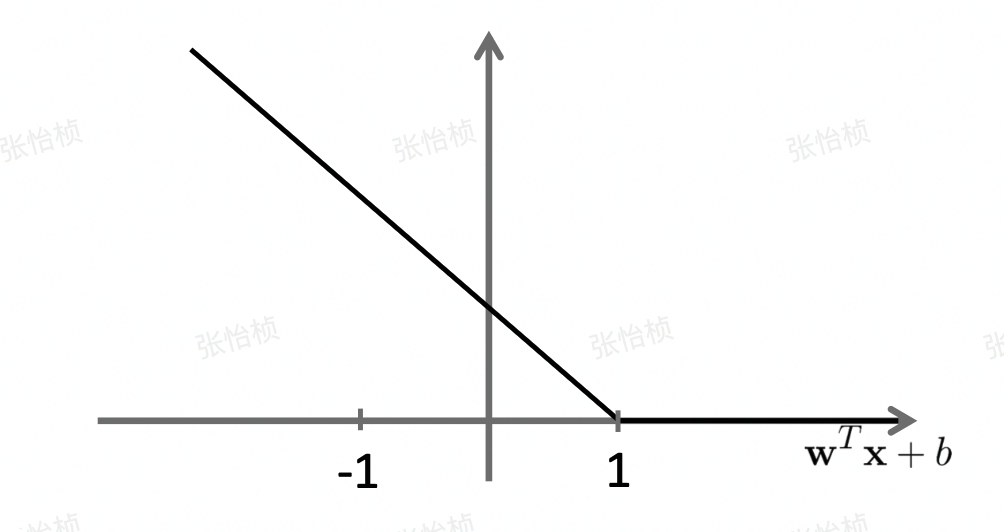
\includegraphics[scale=0.5]{figs/4.png} 
		\caption{Hinge Loss}
		\label{fig:Hinge}
	 \end{figure}

	 \1 样本约束

	 原来的样本严格的约束在$y_{i}\left(\mathbf{w}^{\mathbf{T}_{i}}+b\right) \geqslant 1$
	 现在的样本可以允许一些数据进入margin,这将反映在对结构风险部分的调整
	 \begin{equation}
		y_{i}\left(\mathbf{w}^{\mathbf{T}} \mathbf{x}_{i}+b\right) \geqslant 1-\xi_{i}, \quad \xi_{i} \geq 0, i=1,2, \cdots, m
	 \end{equation}

	 \1 结构风险(未使用拉格朗日乘子法的代价函数)
	
	 该部分引入松弛变量,让一些数据样本可以进入margin,但是对于松弛变量也要做严格的最小化处理
	 \begin{equation}
		 \begin{array}{ll}
			 \min _{\mathbf{w}, b, \xi_{i}} & \frac{1}{2}\|\mathbf{w}\|^{2}+C \sum_{i=1}^{m} \xi_{i} \\
			 \text { s.t. } & y_{i}\left(\mathbf{w}^{\mathbf{T}} \mathbf{x}_{i}+b\right) \geqslant 1-\xi_{i} \\
			 & \xi_{i} \geqslant 0, i=1,2, \cdots, m
			 \end{array}
	 \end{equation}

	 \1 代价函数(使用拉格朗日乘子法)

	 对上述的结构风险与经验风险进行调整后:

	 \begin{equation}
		\min _{\boldsymbol{w}, b, \boldsymbol{\alpha}, \boldsymbol{\xi}, \boldsymbol{\mu}} \frac{1}{2}\|\boldsymbol{w}\|^{2}+\sum_{i=1}^{m} \alpha_{i}\left(1-\xi_{i}-y_{i}\left(\boldsymbol{w}^{T} \boldsymbol{x}_{i}+b\right)\right)+C \sum_{i=1}^{m} \xi_{i}-\sum_{i=1}^{m} \mu_{i} \xi_{i}
	 \end{equation}

	 \1 对代价函数进行优化的优化模型

	 \begin{equation}
		\max _{\alpha}\{ \min _{\mathbf{w}, b, \boldsymbol{\xi}, \boldsymbol{\mu}} L(\mathbf{w}, b, \boldsymbol{\alpha}, \boldsymbol{\xi}, \boldsymbol{\mu})\}
	\end{equation}

	求导后的优化结果:

	\begin{equation}
		\begin{aligned}
			&\max _{\alpha} \min _{\mathbf{w}, b, \boldsymbol{\xi}, \boldsymbol{\mu}} L(\mathbf{w}, b, \boldsymbol{\alpha}, \boldsymbol{\xi}, \boldsymbol{\mu})=\max _{\alpha} \sum_{i=1}^{m} \alpha_{i}-\frac{1}{2} \sum_{i=1}^{m} \sum_{j=1}^{m} \alpha_{i} \alpha_{j} y_{i} y_{j} \mathbf{x}_{i}^{T} \mathbf{x}_{j} \\
			&\text { s.t. } \sum_{i=1}^{m} \alpha_{i} y_{i}=0  ,\quad 0 \leqslant \alpha_{i} \leqslant C, i=1,2, \cdots, m
			\end{aligned}
	\end{equation}

\end{outline}

\subsection{AdaBoost}
\begin{outline}
	\1 损失函数

	使用指数函数作为损失函数
	\begin{equation}\label{loss:16}
		L(y, f(x))=e^{-y f(x)}
	 \end{equation}



	\1 代价函数

	若将指数损失表示为期望值的形式:
	\begin{equation}
		E\left(e^{-y f(x)} \mid x\right)=P(y=1 \mid x) e^{-f(x)}+P(y=-1 \mid x) e^{f(x)}
	\end{equation}
	\begin{figure}[h]%  figure placement
		\centering
		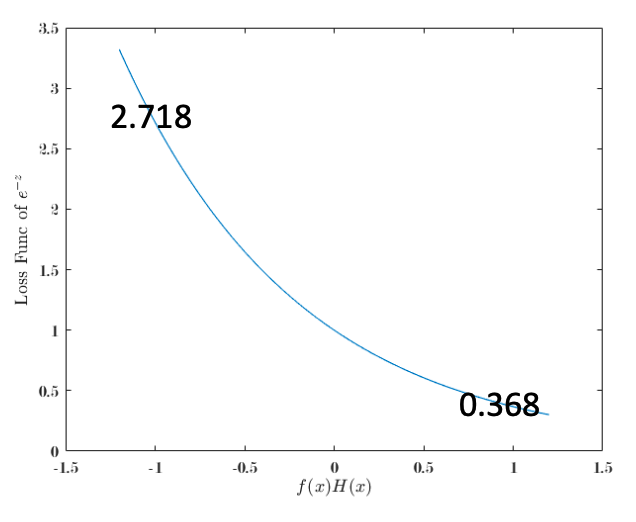
\includegraphics[scale=0.8]{figs/5.png} 
		\caption{Exponential Loss}
		\label{fig:Exponential}
	 \end{figure}

\end{outline}


% ----------------------------- %
% References:  BibTeX
% ----------------------------- %
%\bibliography{refs.bib}
%\bibliographystyle{apalike}


\end{document} 
